\documentclass[12pt]{article}

\usepackage{sbc-template}

\usepackage{graphicx,url}

%\usepackage[brazil]{babel}   
\usepackage[latin1]{inputenc}  

     
\sloppy

\title{Desenvolvimento de uma Ontologia para o Dom�nio de Engenharia de Software}

\author{Jamile Almeida\inst{1}, Lorena S. Pereira\inst{1}, Rog�rio do Carmo\inst{1}, Thiago Jos� Alvoravel\inst{1}}


\address{Colegiado de Sistemas de Informa��o - Universidade do Estado da Bahia (UNEB)\\
  Caixa Postal 41.150-000 - Salvador - BA - Brazil
  \email{ \{jamileferreira1313, lorena.santpe, rogersineb, t.alvoravel\}@gmail.com}
}

\begin{document} 

\maketitle

\begin{abstract}
  To do
\end{abstract}
     
\begin{resumo} 
  To do
\end{resumo}


\section{Introdu��o}


\section{Representa��o do Conhecimento}


\subsection{Taxonomia}


\subsection{Tesauro}


\subsection{Classifica��o Facetada}


\section{Metodologia}

\section{Trabalhos Correlatos}


\begin{figure}[ht]
\centering
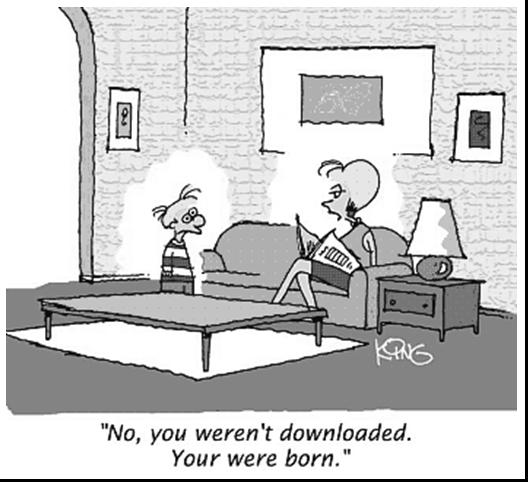
\includegraphics[width=.5\textwidth]{fig1.jpg}
\caption{A typical figure}
\label{fig:exampleFig1}
\end{figure}

\section{Refer�ncias}


\bibliographystyle{sbc}
\bibliography{sbc-template}

\end{document}
